
        \begin{figure}[H]
            \centering
            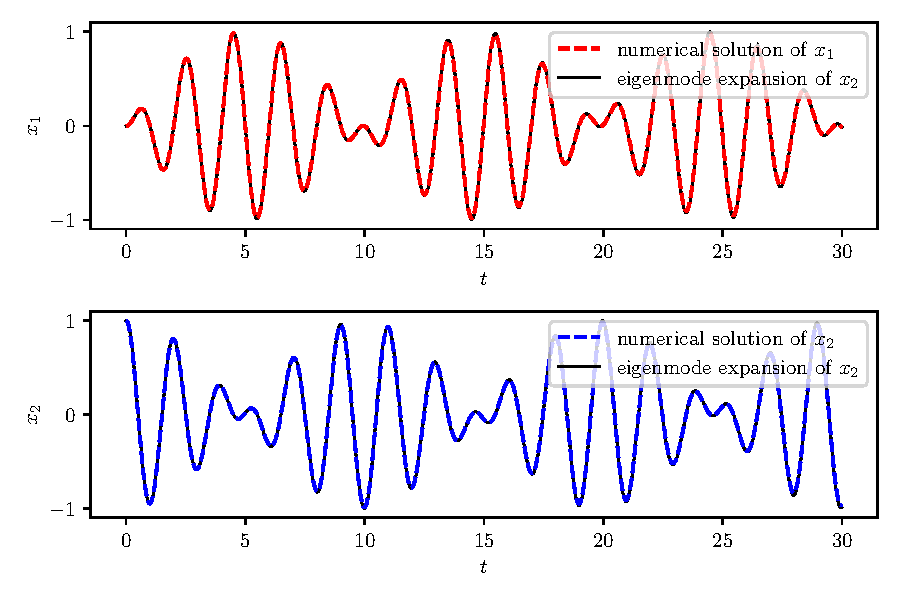
\includegraphics[width=0.9\linewidth]{../Numerical-Calculation/img/(k1,k2,k3)=(4.0,1.0,4.0),(m1,m2)=(0.5,0.5),(x1_i,x1_2)=(0.0,1.0).pdf}
            \caption{Motion curve for $\left(k_1,k_2,k_3\right)=\left(4.0,1.0,4.0\right)$, $\left(m_1,m_2\right)=\left(0.5,0.5\right)$ and the intial consition $\left(x_{1}(0),x_2(0)\right)=\left(0.0,-1.0\right)$}
        \end{figure}

        \begin{figure}[H]
            \centering
            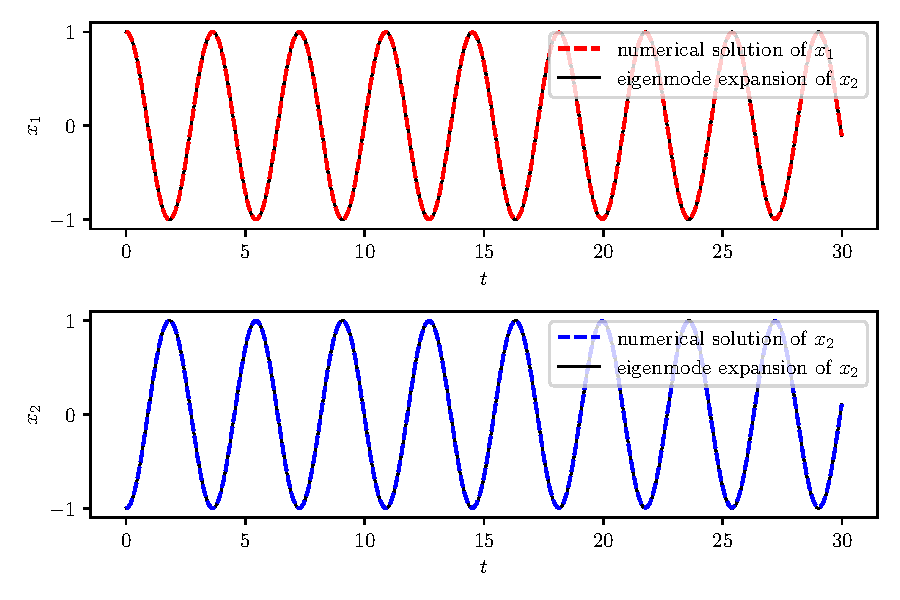
\includegraphics[width=0.9\linewidth]{../Numerical-Calculation/img/(k1,k2,k3)=(1.0,1.0,1.0),(m1,m2)=(1.0,1.0),(x1_i,x1_2)=(1.0,-1.0).pdf}
            \caption{Motion curve for $\left(k_1,k_2,k_3\right)=\left(1.0,1.0,1.0\right)$, $\left(m_1,m_2\right)=\left(1.0,1.0\right)$ and the intial consition $\left(x_{1}(0),x_2(0)\right)=\left(1.0,-1.0\right)$}
        \end{figure}

        \begin{figure}[H]
            \centering
            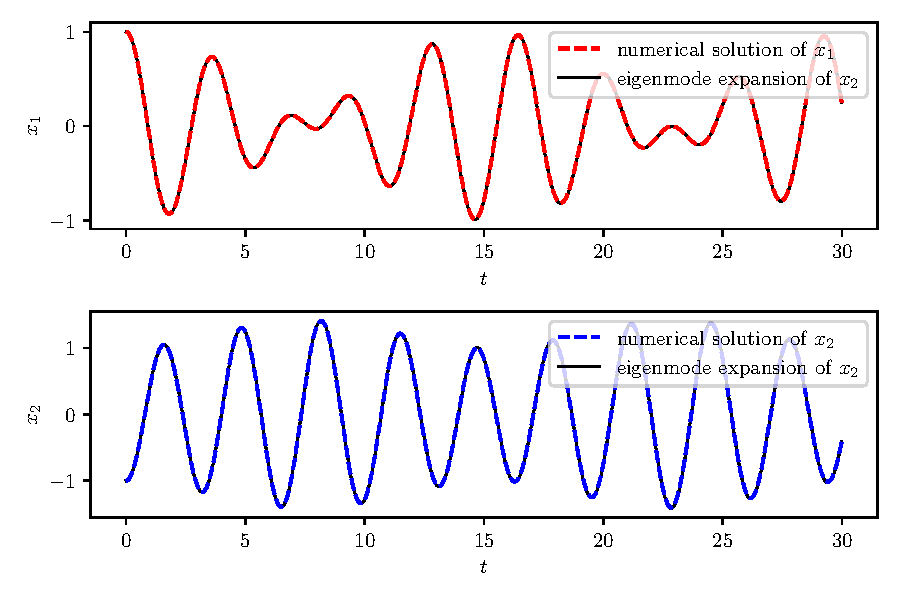
\includegraphics[width=0.9\linewidth]{../Numerical-Calculation/img/(k1,k2,k3)=(2.0,0.5,3.0),(m1,m2)=(1.0,1.0),(x1_i,x1_2)=(1.0,-1.0).pdf}
            \caption{Motion curve for $\left(k_1,k_2,k_3\right)=\left(2.0,0.5,3.0\right)$, $\left(m_1,m_2\right)=\left(1.0,1.0\right)$ and the intial consition $\left(x_{1}(0),x_2(0)\right)=\left(1.0,-1.0\right)$}
        \end{figure}

        \begin{figure}[H]
            \centering
            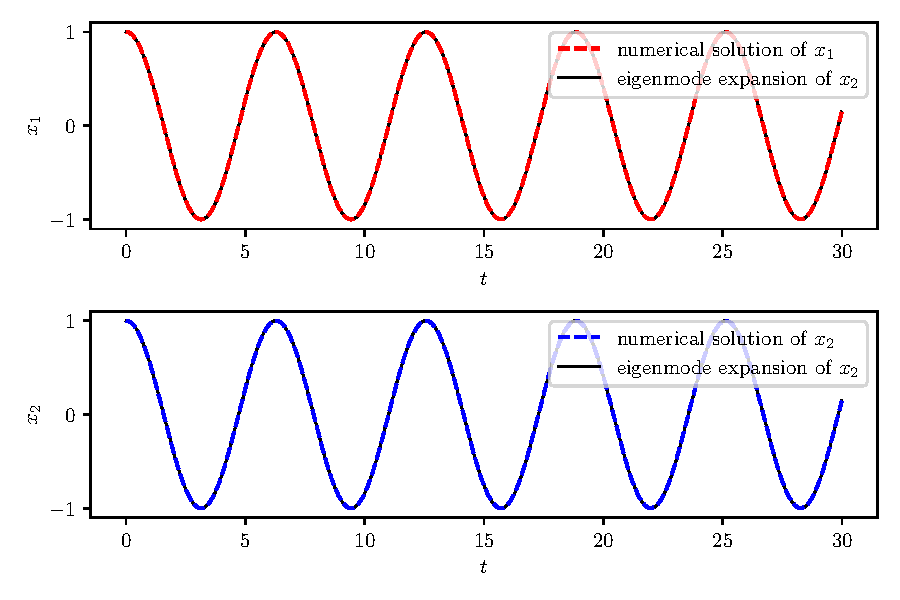
\includegraphics[width=0.9\linewidth]{../Numerical-Calculation/img/(k1,k2,k3)=(1.0,1.0,1.0),(m1,m2)=(1.0,1.0),(x1_i,x1_2)=(1.0,1.0).pdf}
            \caption{Motion curve for $\left(k_1,k_2,k_3\right)=\left(1.0,1.0,1.0\right)$, $\left(m_1,m_2\right)=\left(1.0,1.0\right)$ and the intial consition $\left(x_{1}(0),x_2(0)\right)=\left(1.0,-1.0\right)$}
        \end{figure}
